%----------------------------------------
\begin{frame}
  \frametitle{The Deployment page} \small

\vspace{-0.15cm}
{\centering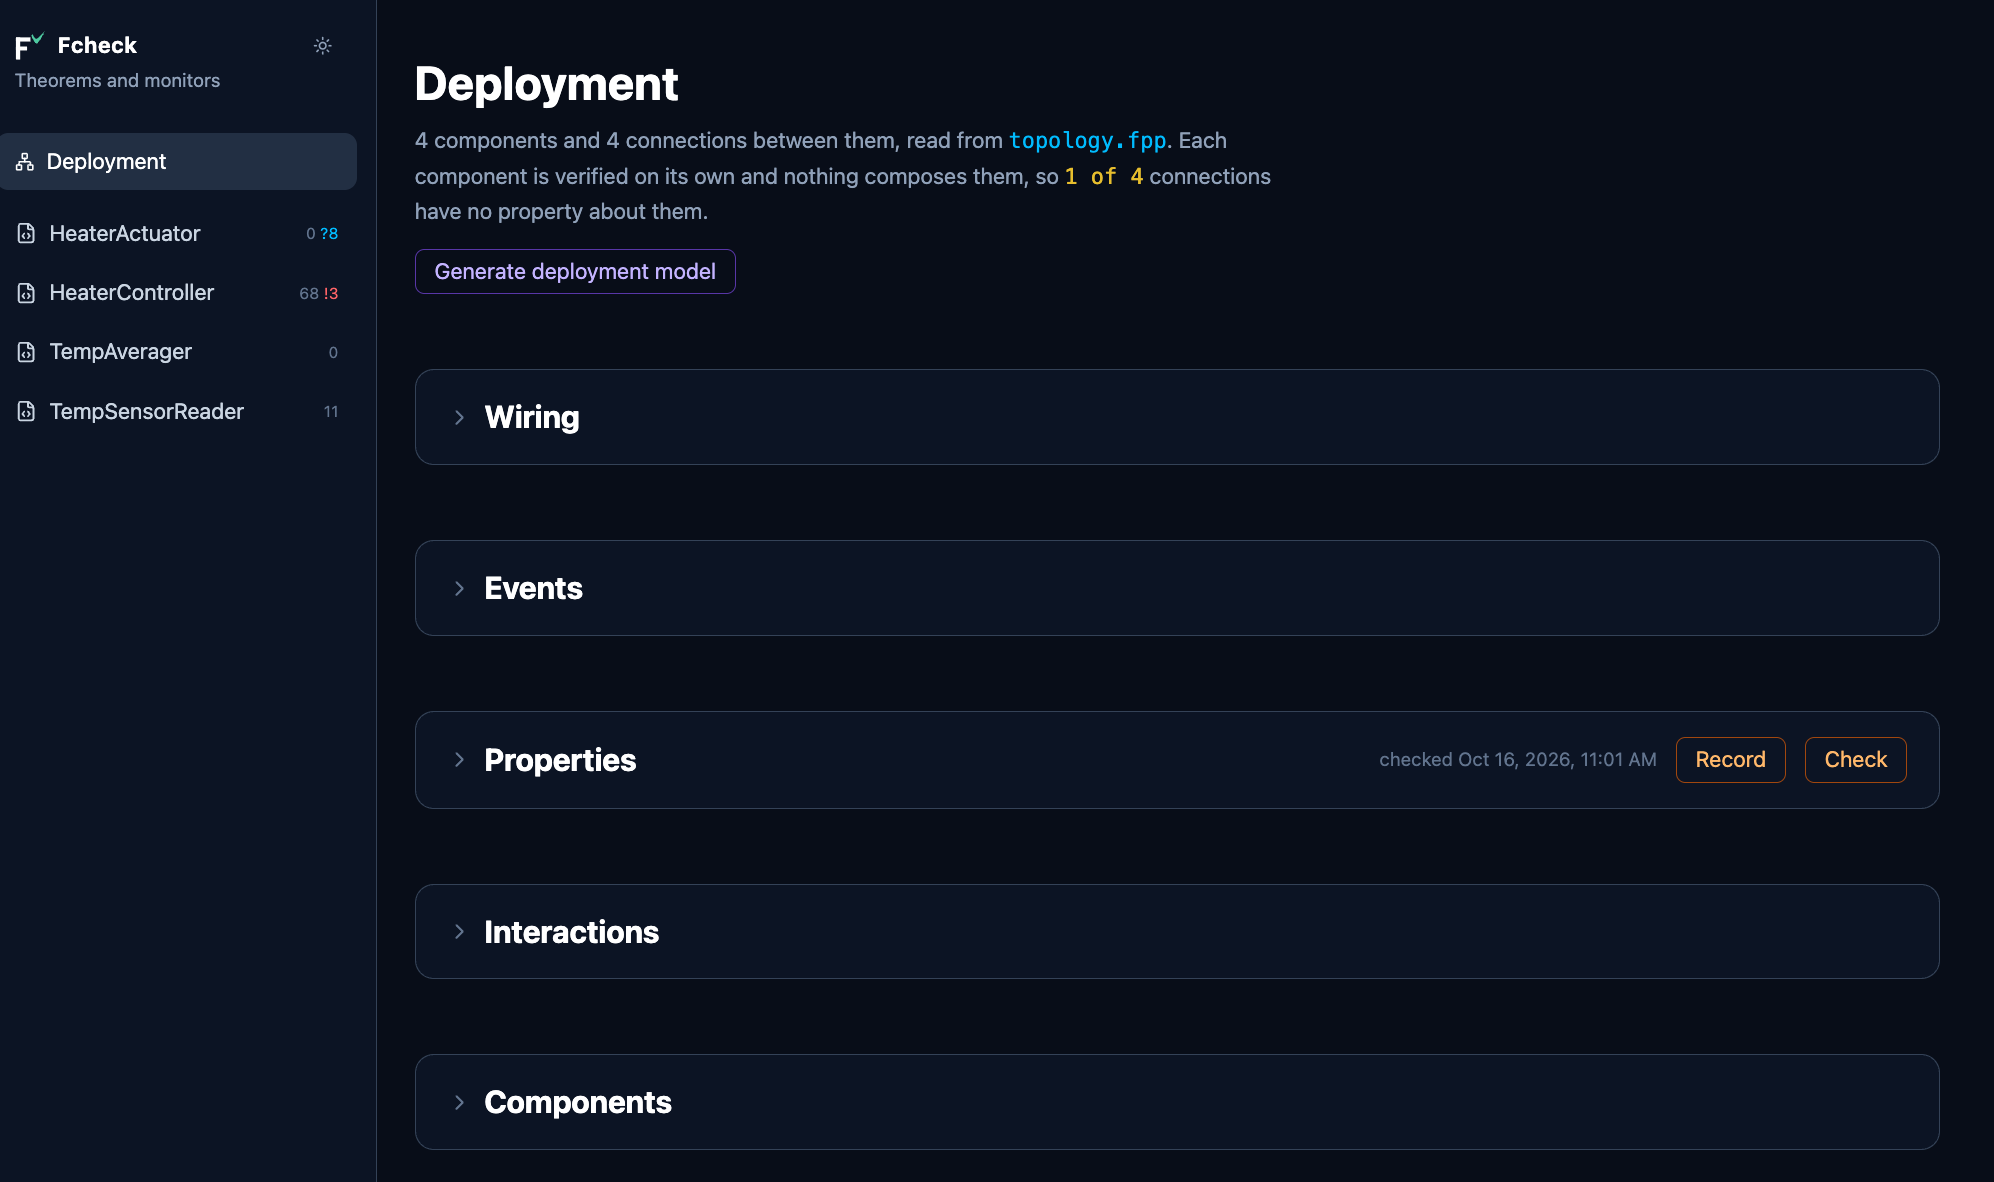
\includegraphics[width=\textwidth,height=0.74\textheight,keepaspectratio]{figures/1-deployment.png}\par}

\vspace{0.1cm}
{\scriptsize Generated from {\tt topology.fpp}}

\end{frame}

%----------------------------------------
\begin{frame}
  \frametitle{The wiring} \small

\vspace{-0.15cm}
{\centering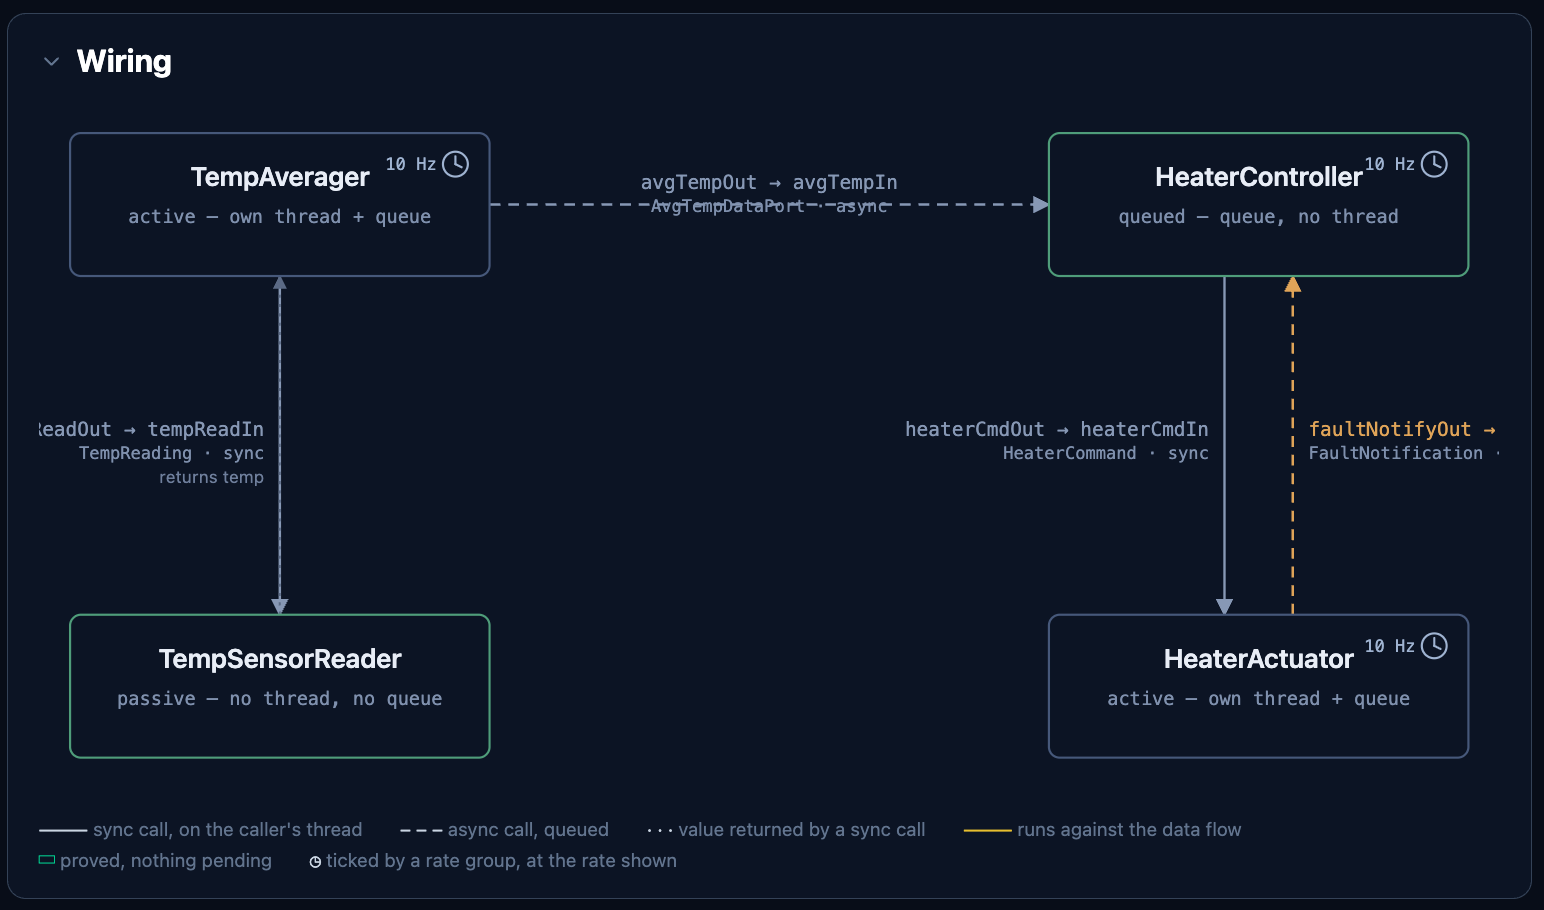
\includegraphics[width=\textwidth,height=0.74\textheight,keepaspectratio]{figures/2-wiring.png}\par}

\vspace{0.1cm}
{\scriptsize Read from the topology: sync and async ports, rate groups, data flow.}

\end{frame}

%----------------------------------------
\begin{frame}
  \frametitle{What temporal properties can talk about} \small

\vspace{-0.15cm}
{\centering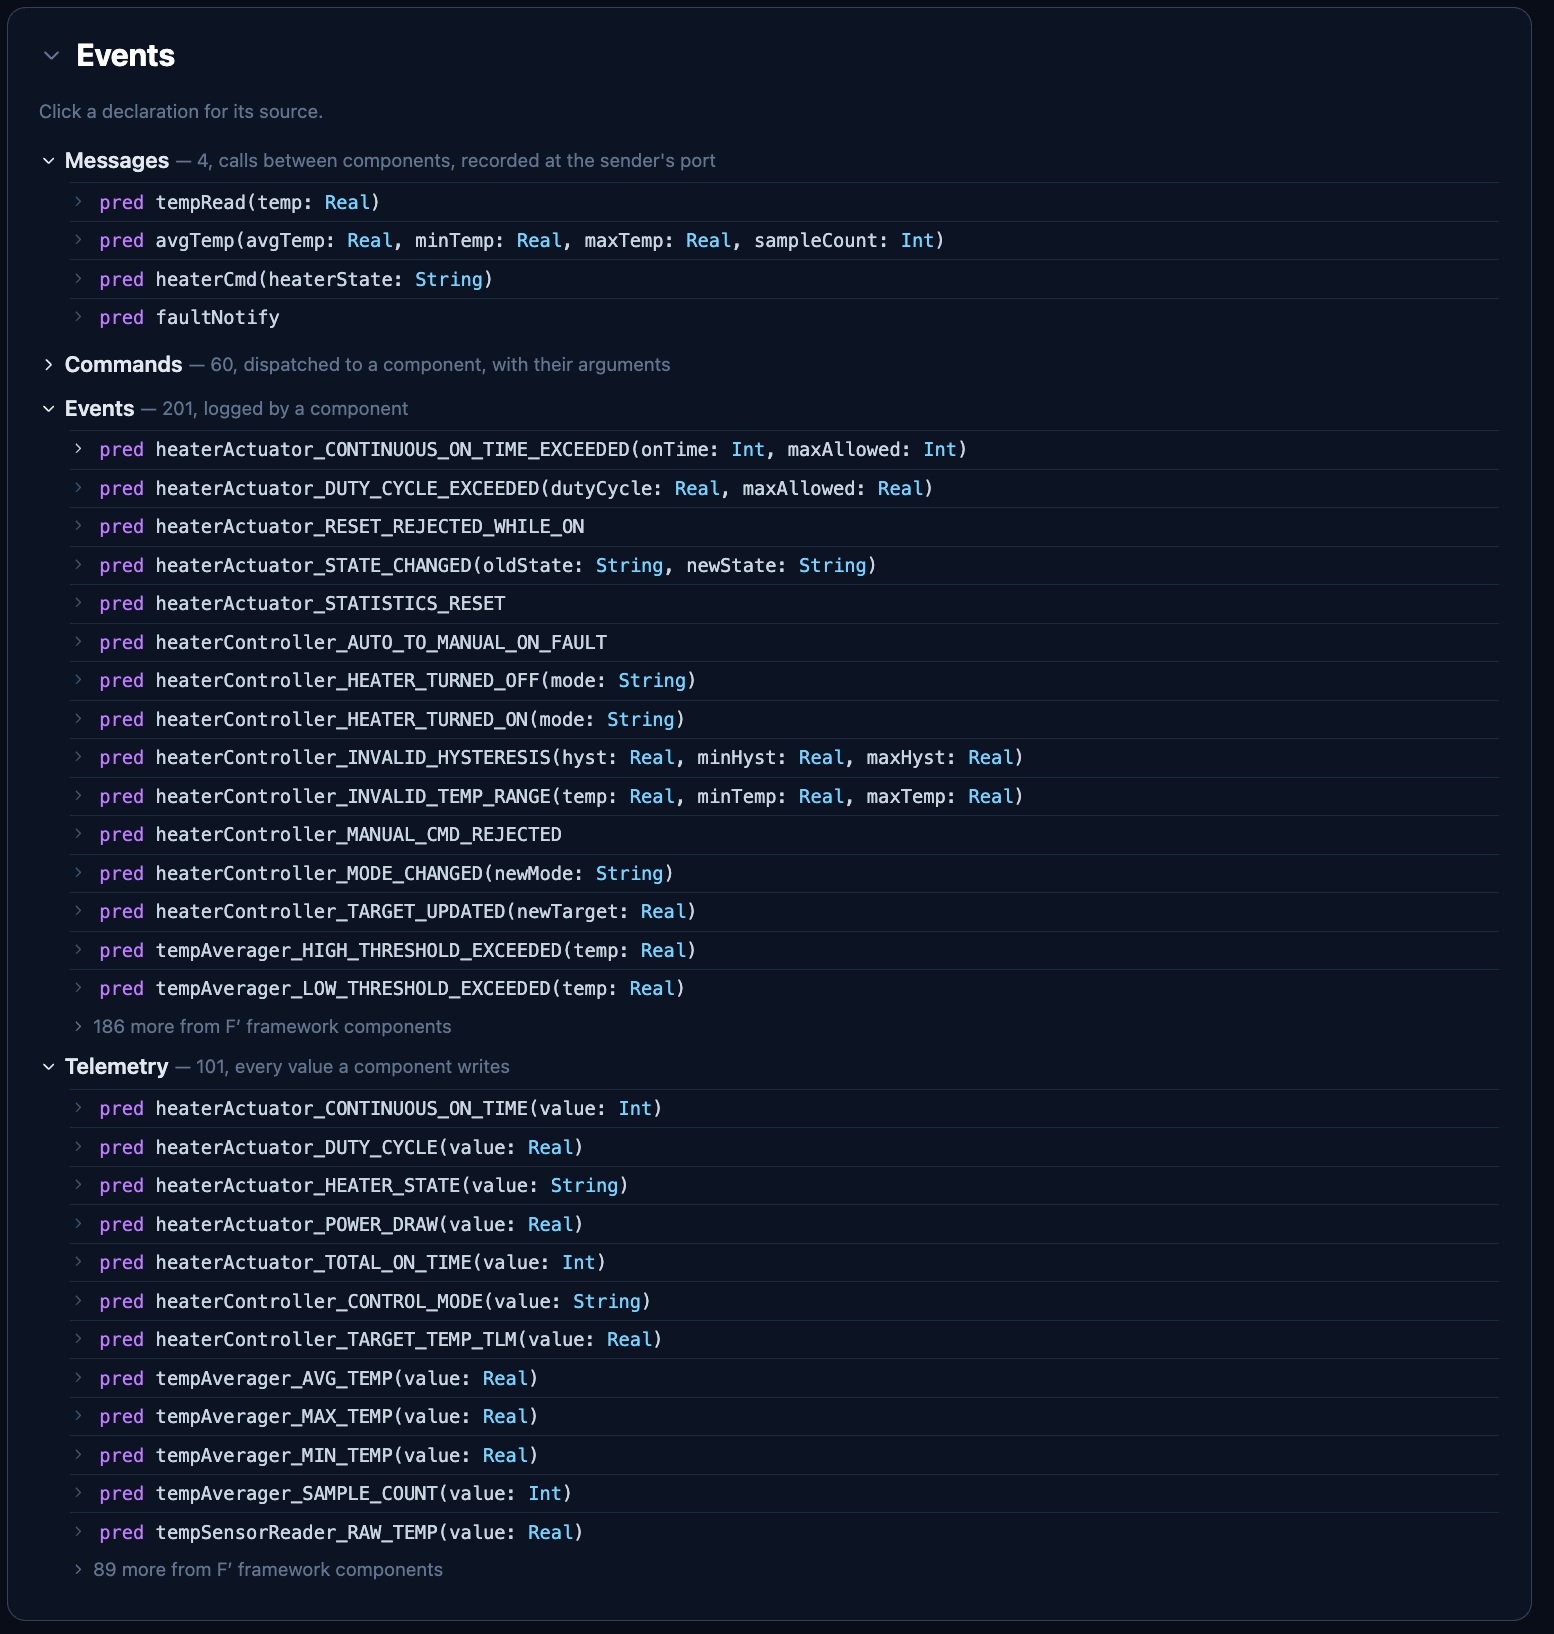
\includegraphics[width=\textwidth,height=0.74\textheight,keepaspectratio]{figures/3-events.png}\par}

\vspace{0.1cm}
{\scriptsize Generated from the \fprime{} dictionary: every message, command, event and telemetry channel, typed.}

\end{frame}

%----------------------------------------
\begin{frame}
  \frametitle{Deployment properties: \dejavumt{}} \small

\vspace{-0.15cm}
{\centering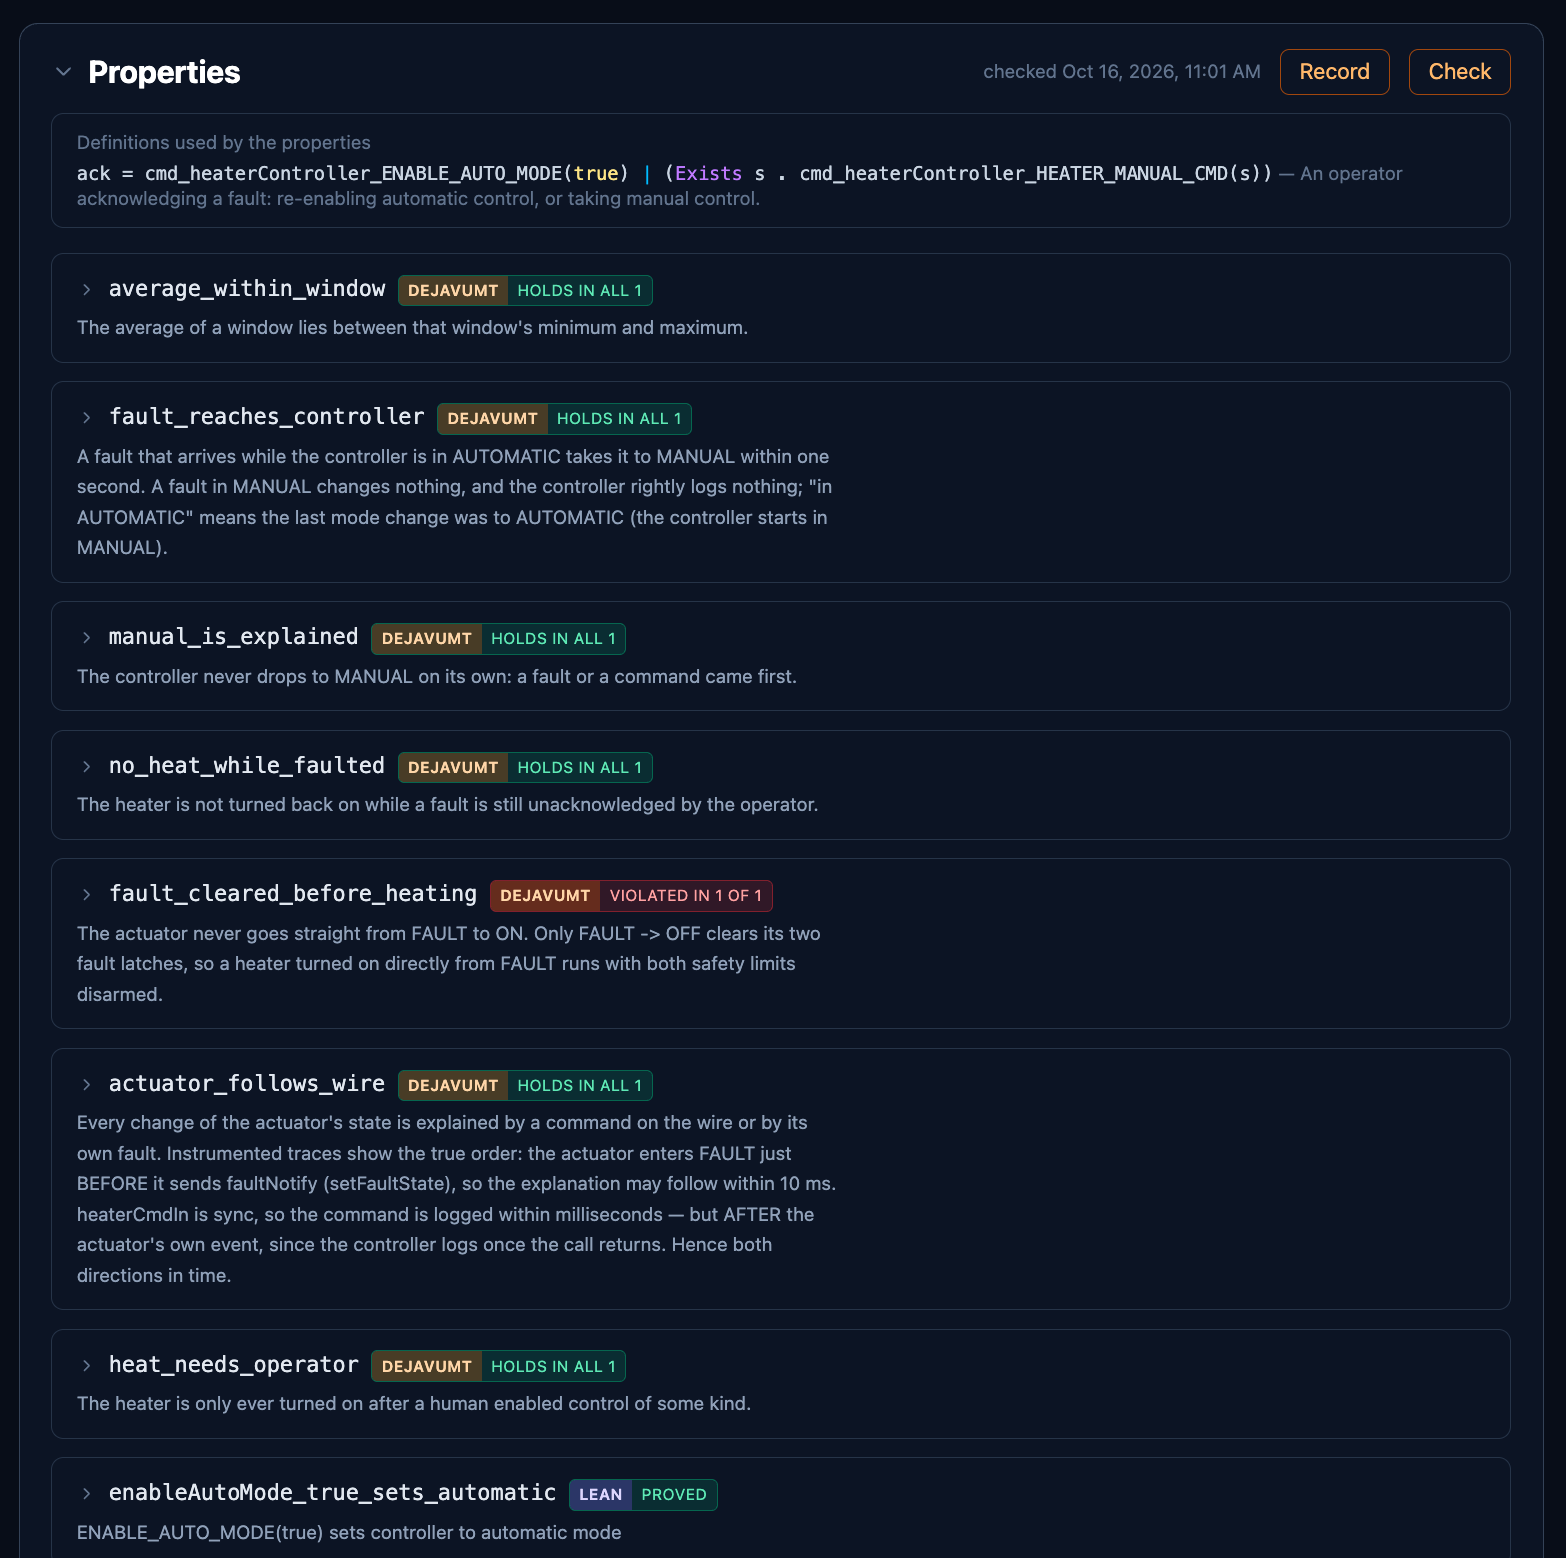
\includegraphics[width=\textwidth,height=0.74\textheight,keepaspectratio]{figures/4-properties1.png}\par}

\vspace{0.1cm}
{\scriptsize Checked on recorded runs of the instrumented system. One is violated.}

\end{frame}

%----------------------------------------
\begin{frame}
  \frametitle{Deployment properties: \lean{}} \small

\vspace{-0.15cm}
{\centering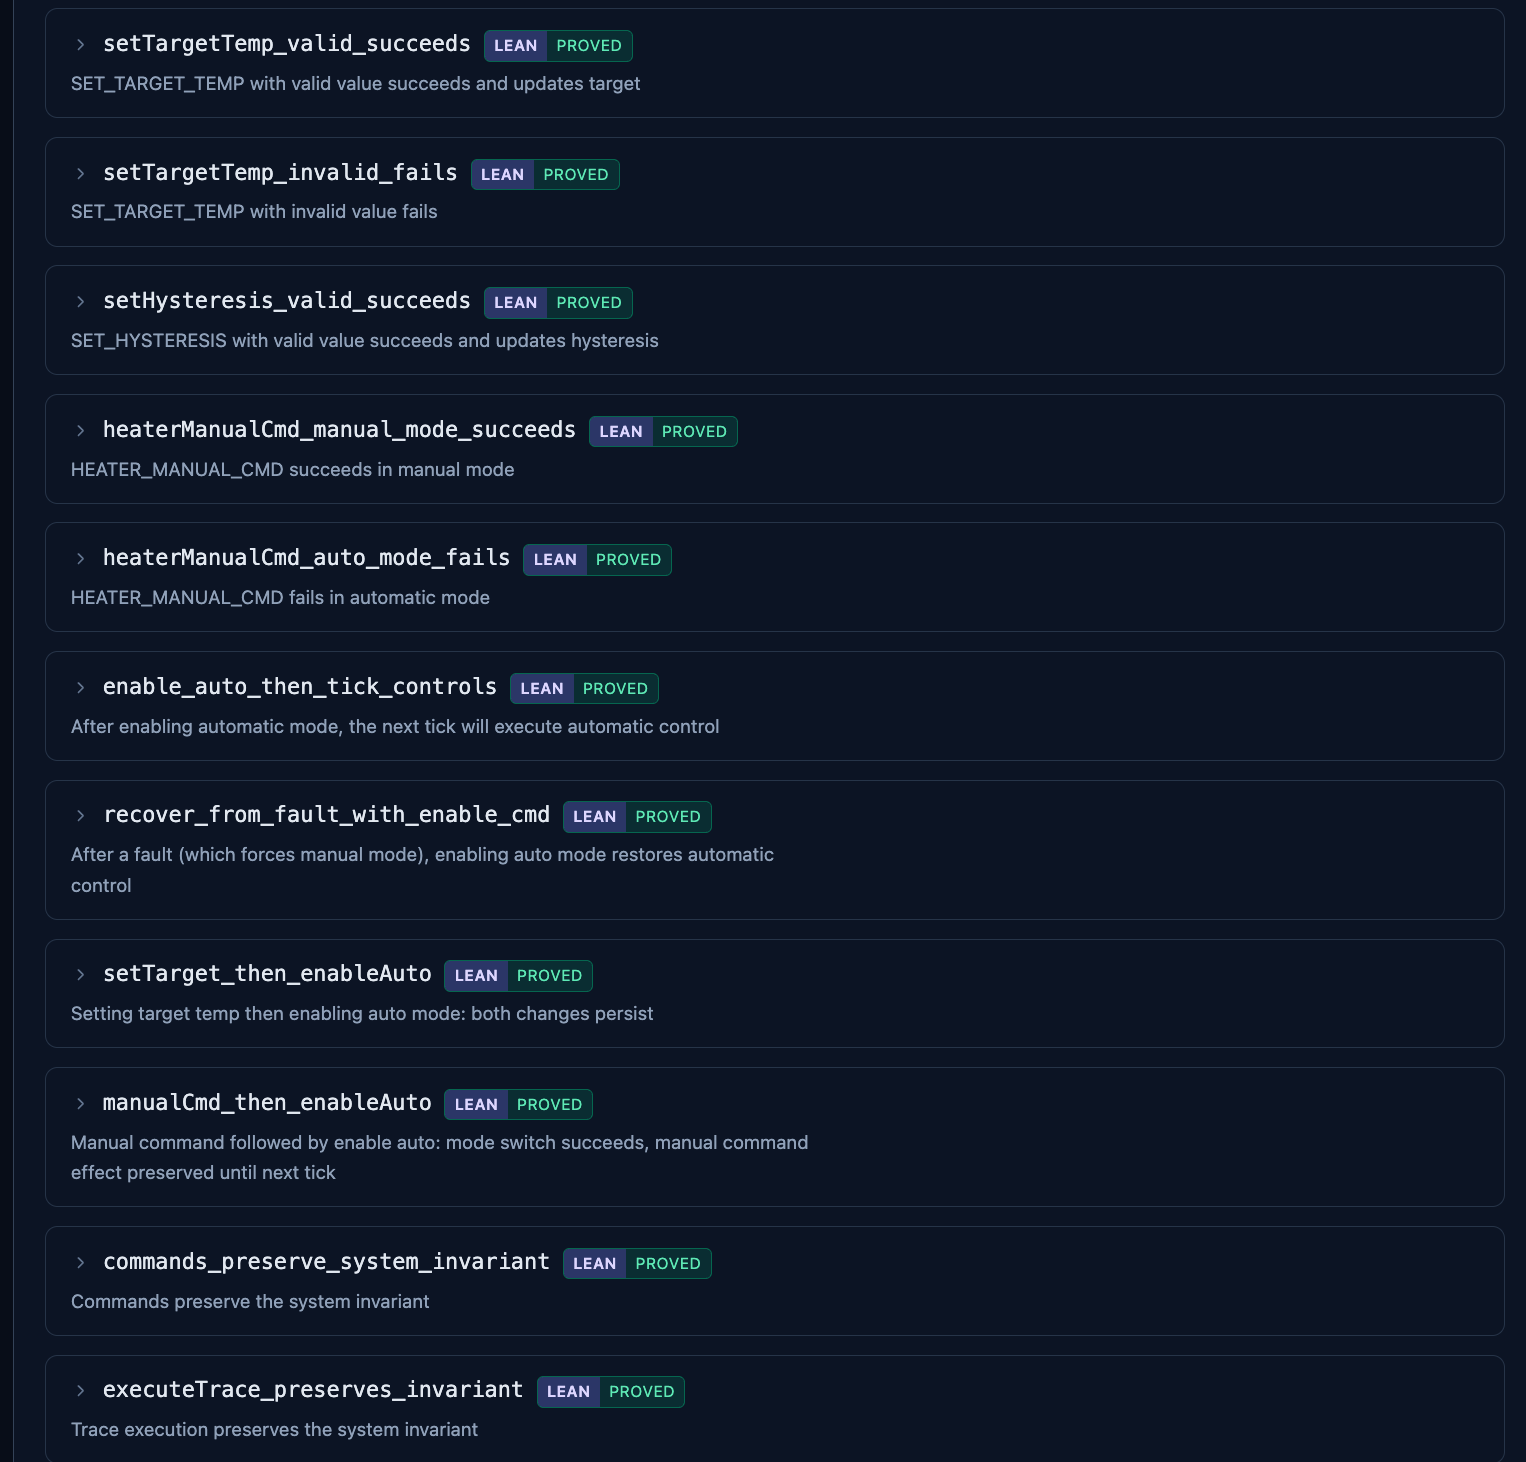
\includegraphics[width=\textwidth,height=0.74\textheight,keepaspectratio]{figures/5-properties2.png}\par}

\vspace{0.1cm}
{\scriptsize Theorems over the system model.}

\end{frame}

%----------------------------------------
\begin{frame}
  \frametitle{A component page} \small

\vspace{-0.15cm}
{\centering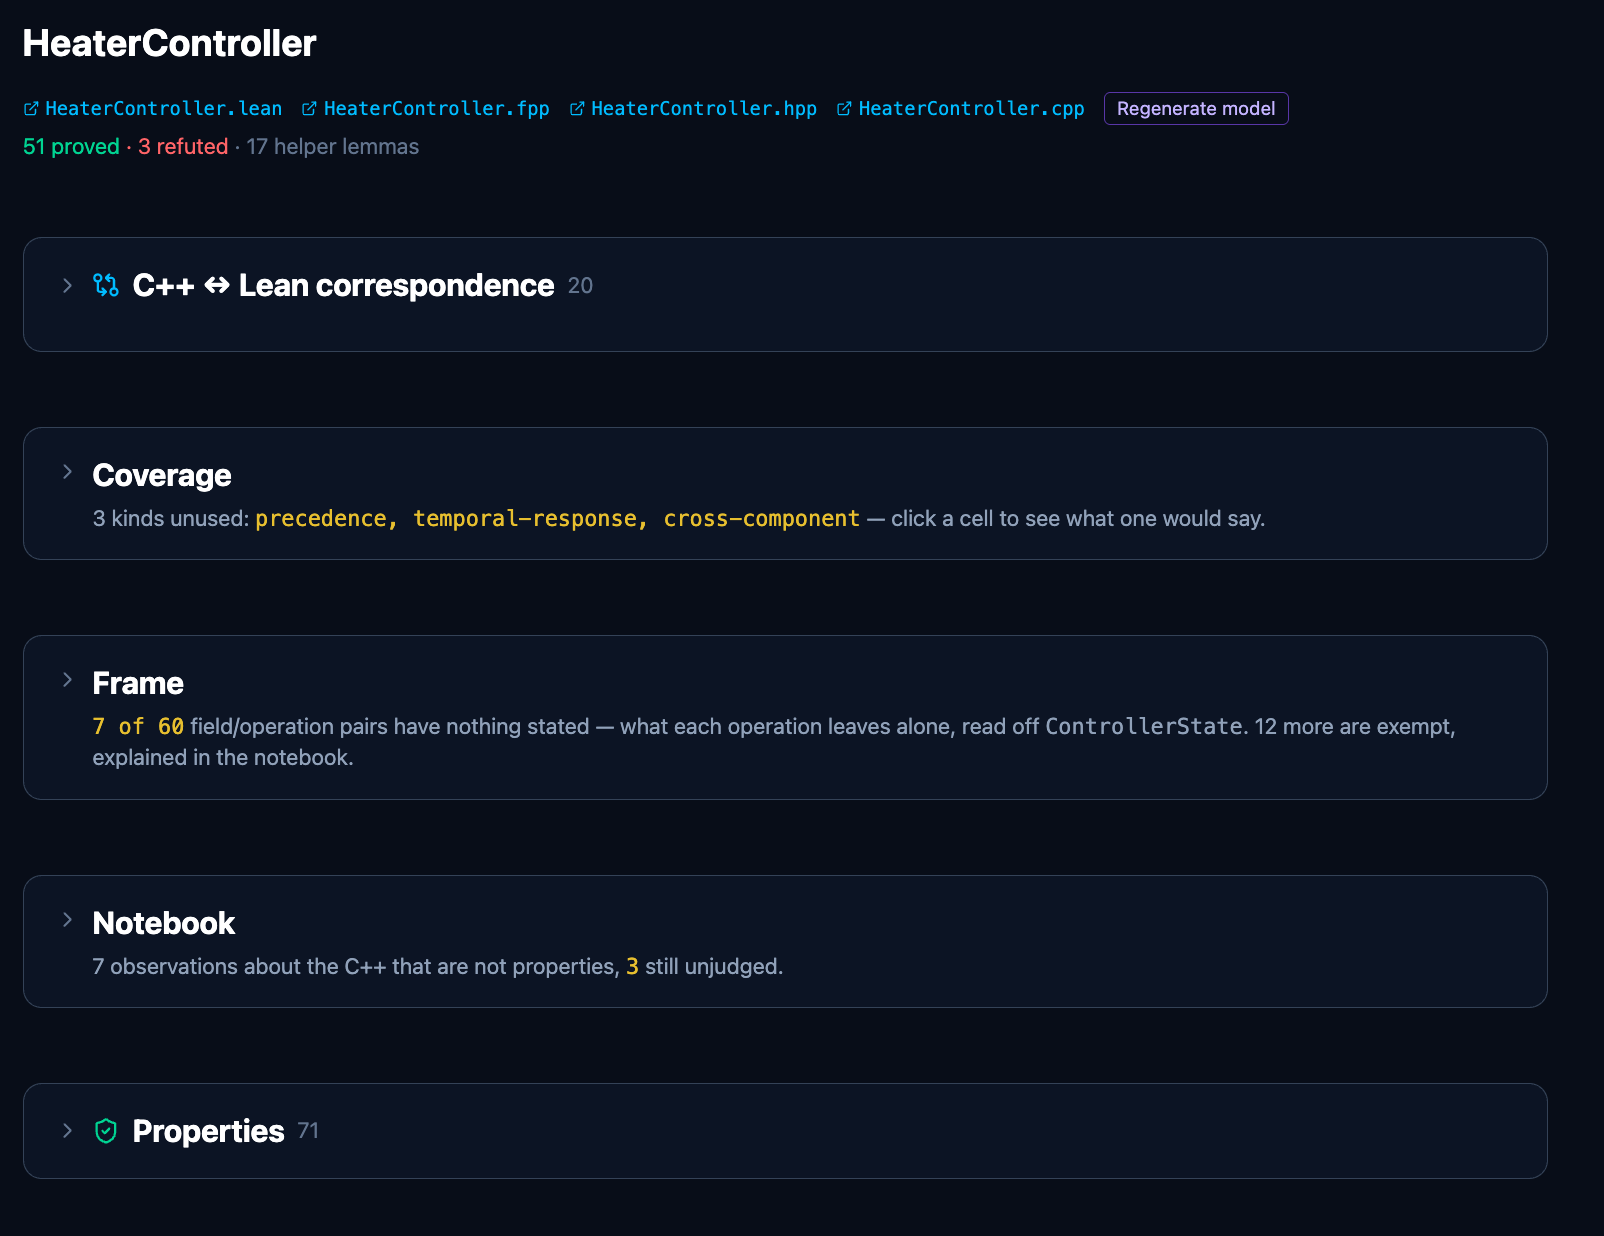
\includegraphics[width=\textwidth,height=0.74\textheight,keepaspectratio]{figures/6-heatercontroller.png}\par}

\end{frame}

%----------------------------------------
\begin{frame}
  \frametitle{The C++ $\leftrightarrow$ \lean{} correspondence} \small

\vspace{-0.15cm}
{\centering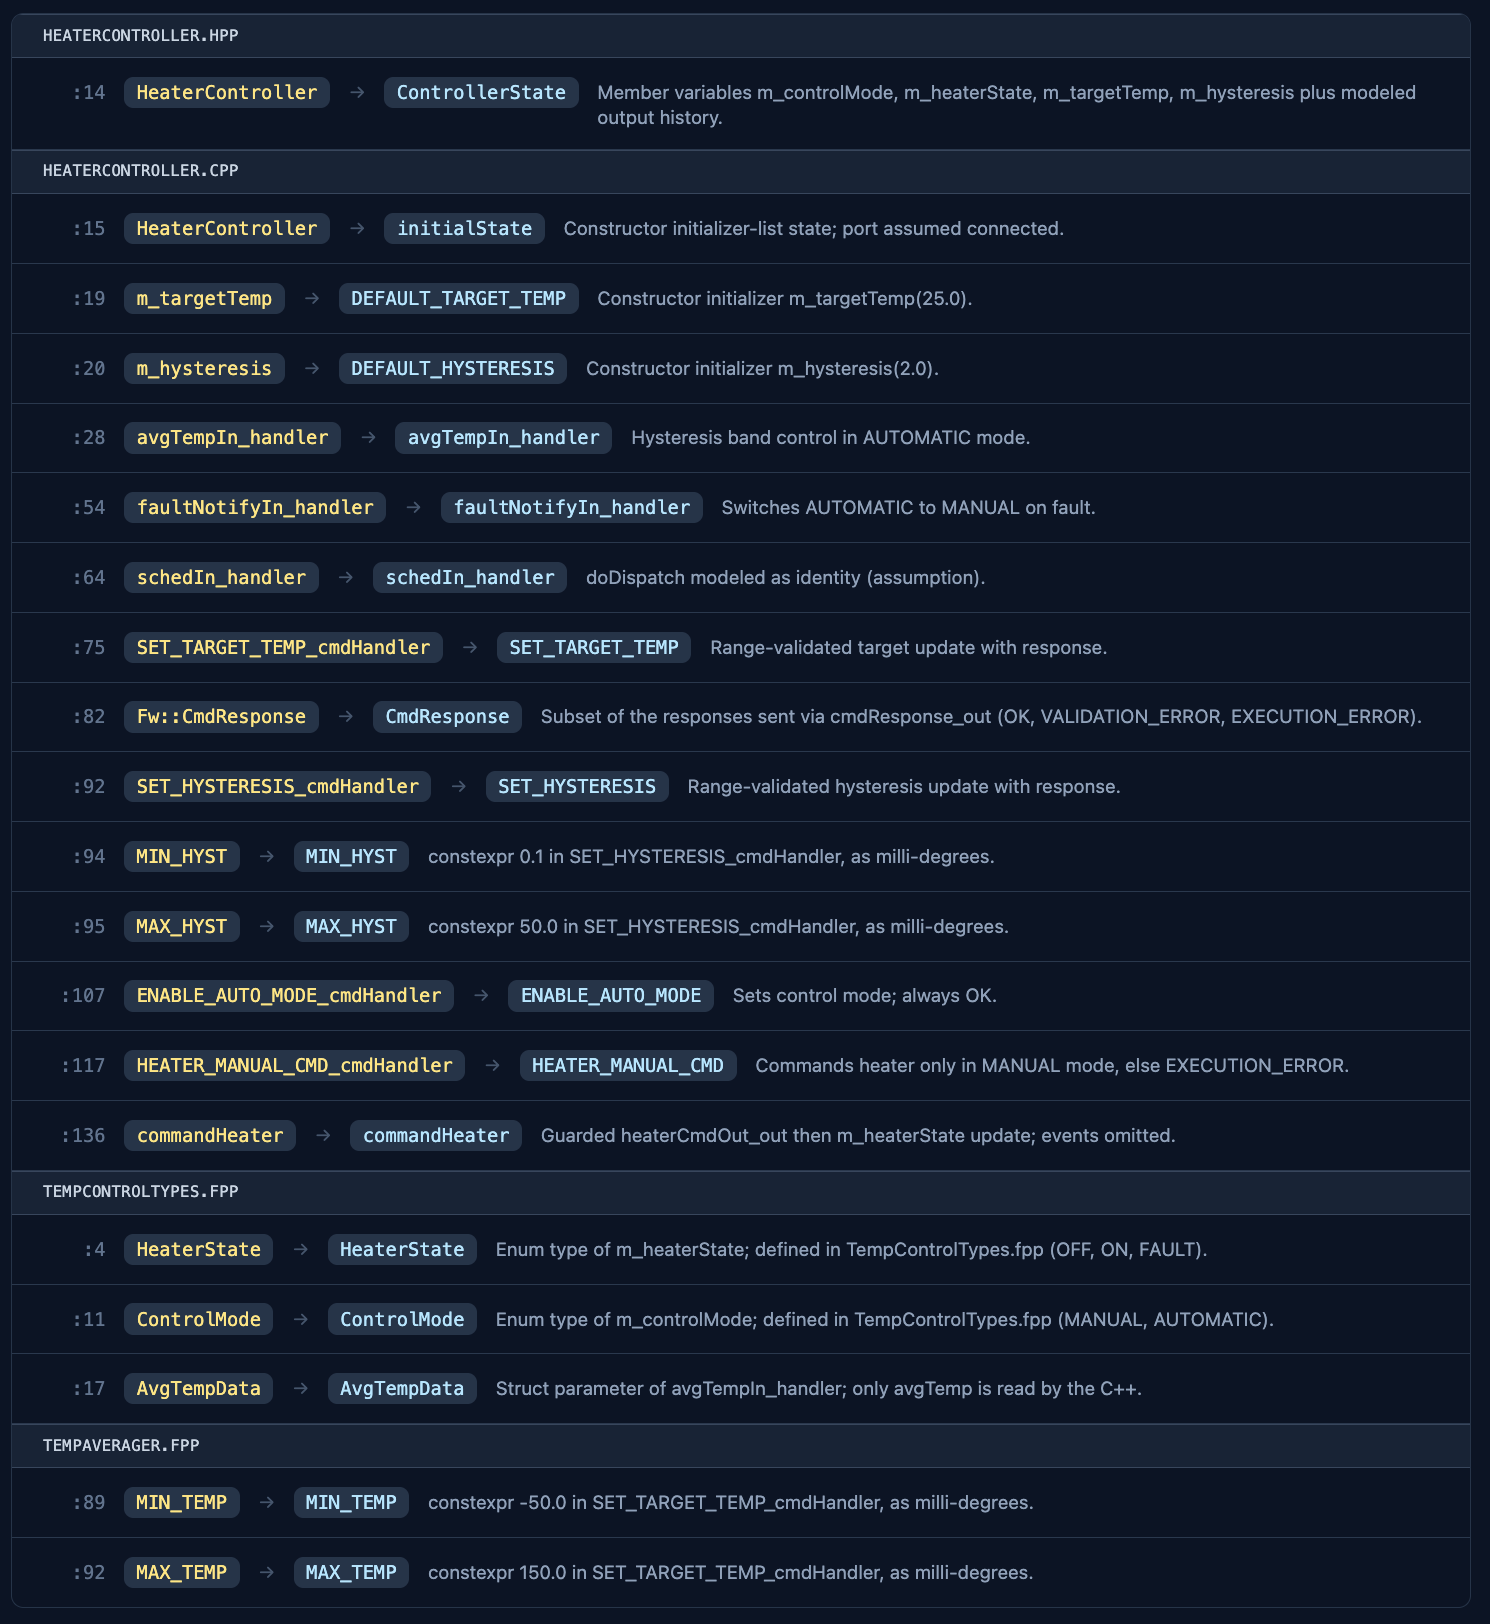
\includegraphics[width=\textwidth,height=0.74\textheight,keepaspectratio]{figures/7-cpp-lean.png}\par}

\vspace{0.1cm}
{\scriptsize What each C++ element became in the model.}

\end{frame}

%----------------------------------------
\begin{frame}
  \frametitle{Clicking a row opens both sides} \small

\vspace{-0.15cm}
{\centering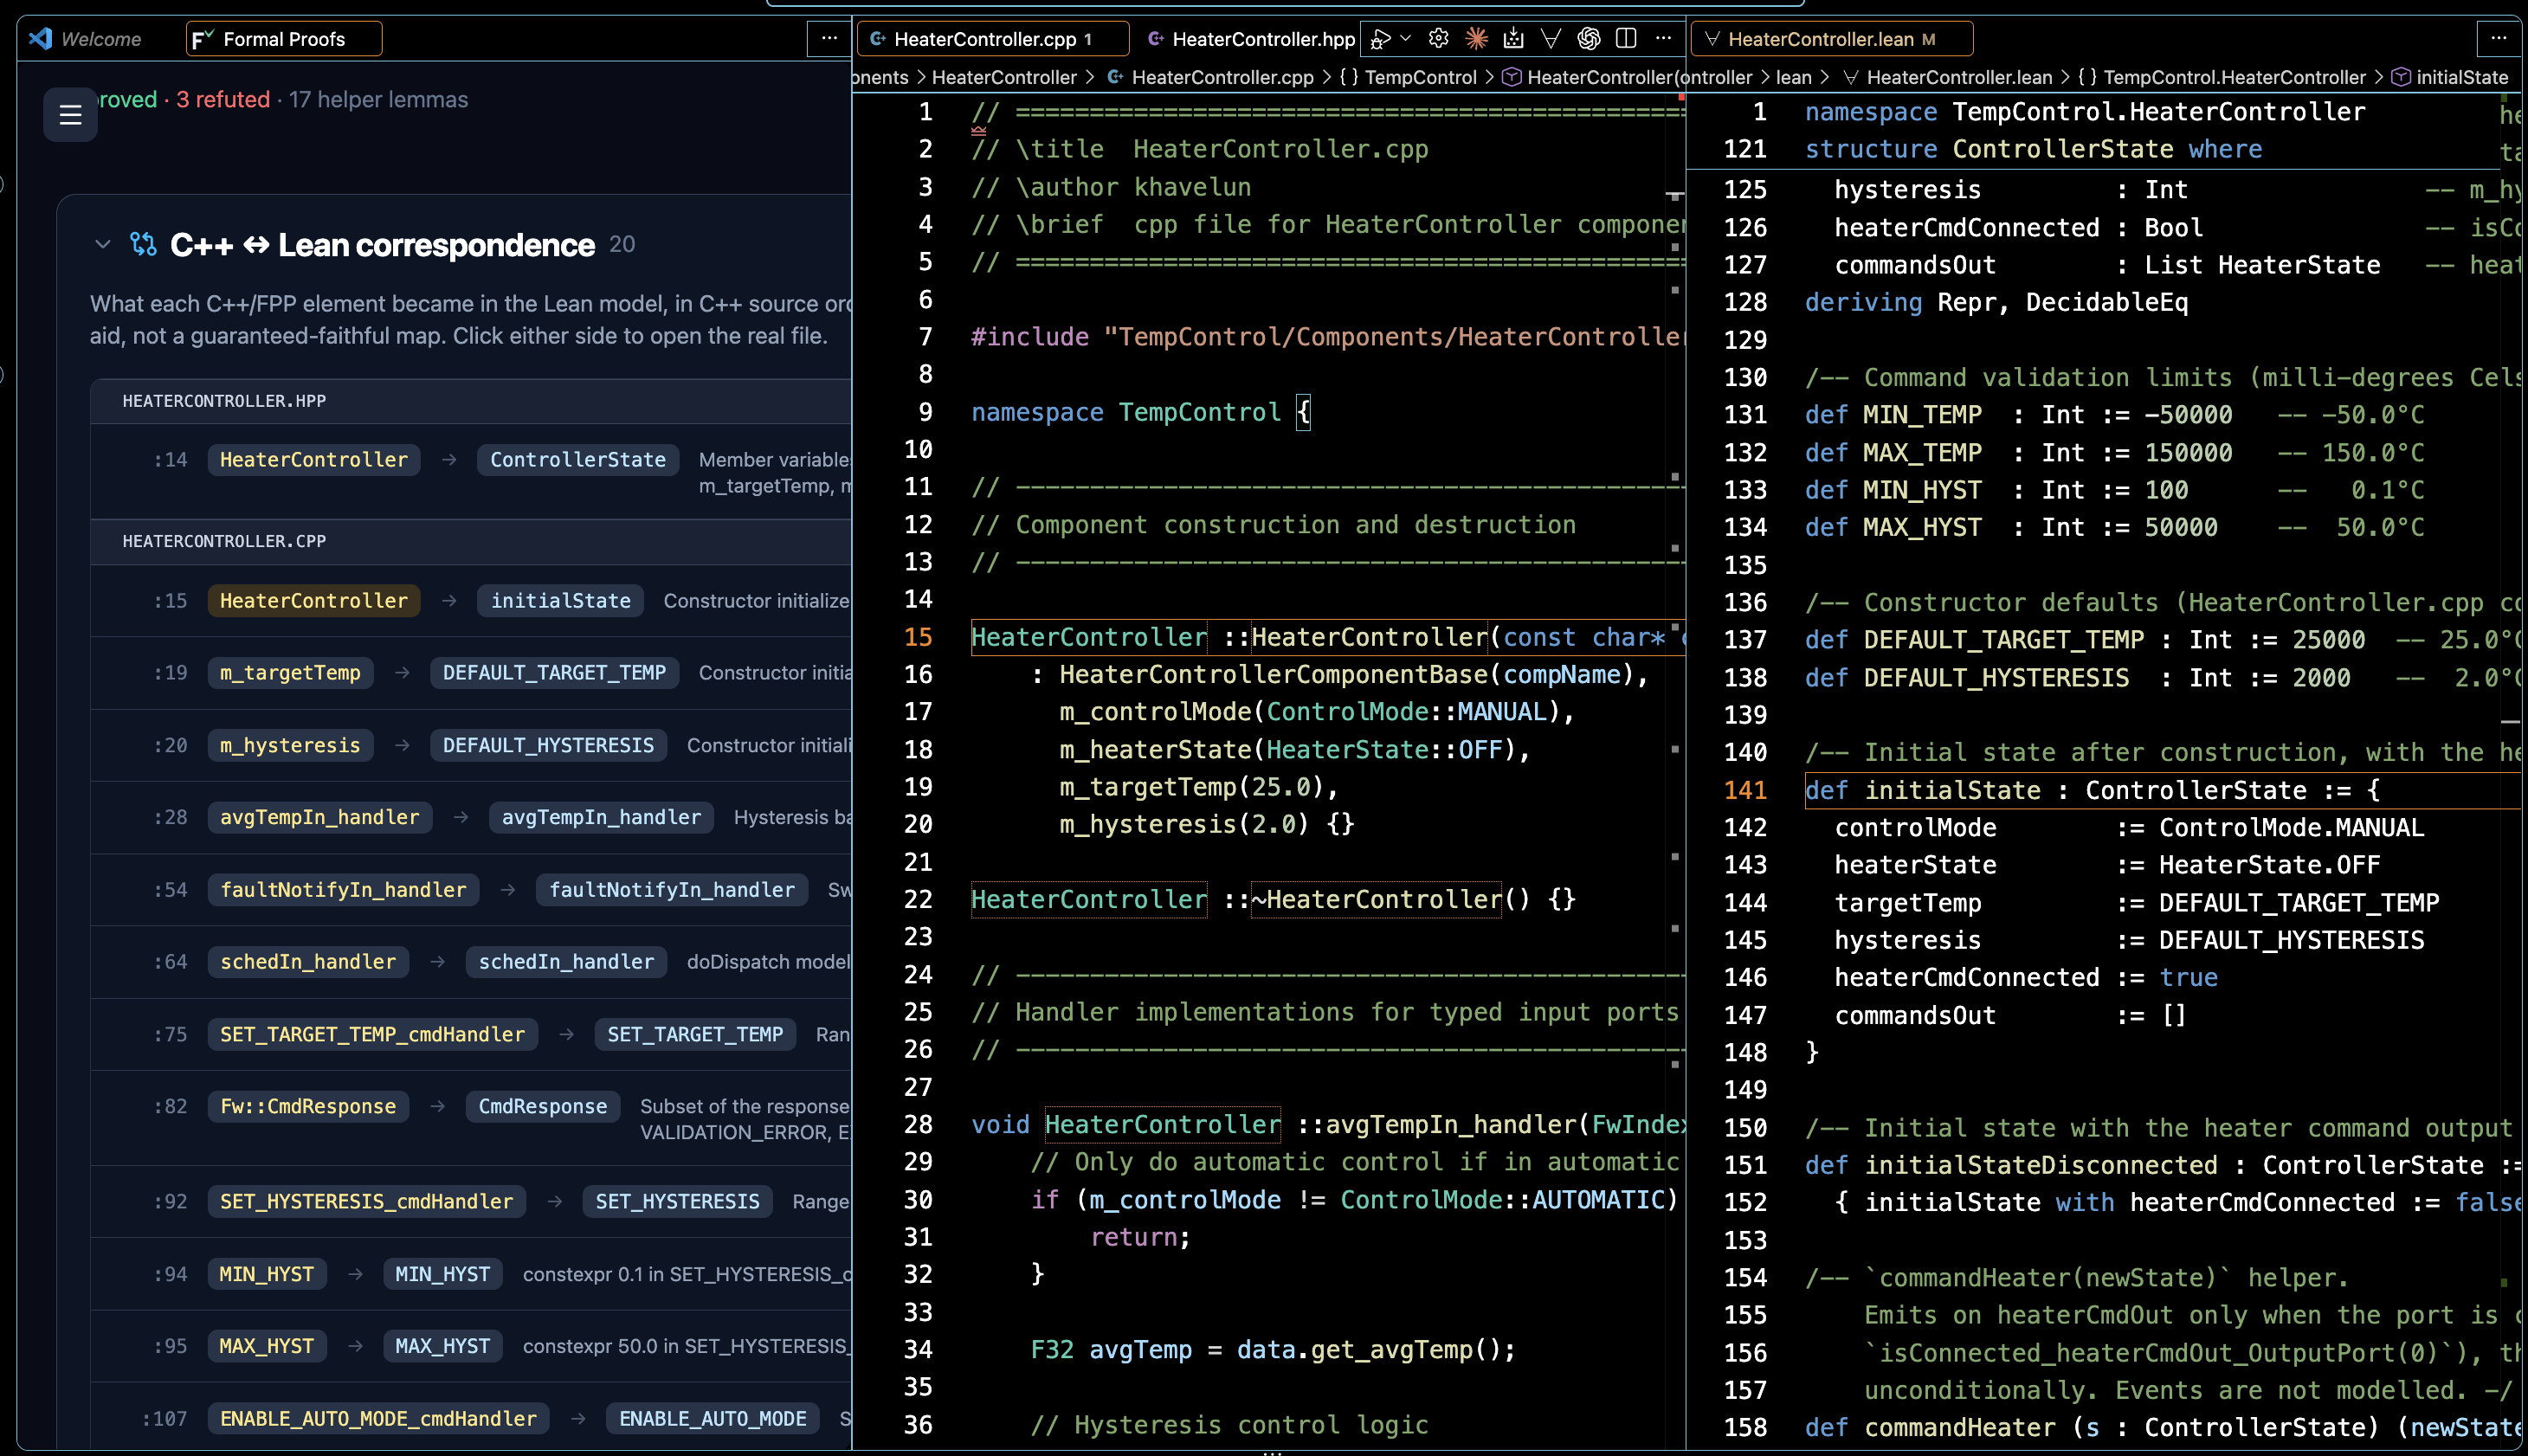
\includegraphics[width=\textwidth,height=0.74\textheight,keepaspectratio]{figures/8-init-state.png}\par}

\vspace{0.1cm}
{\scriptsize The C++ constructor and the \lean{} {\tt initialState}, side by side.}

\end{frame}

%----------------------------------------
\begin{frame}
  \frametitle{The handler and its model} \small

\vspace{-0.15cm}
{\centering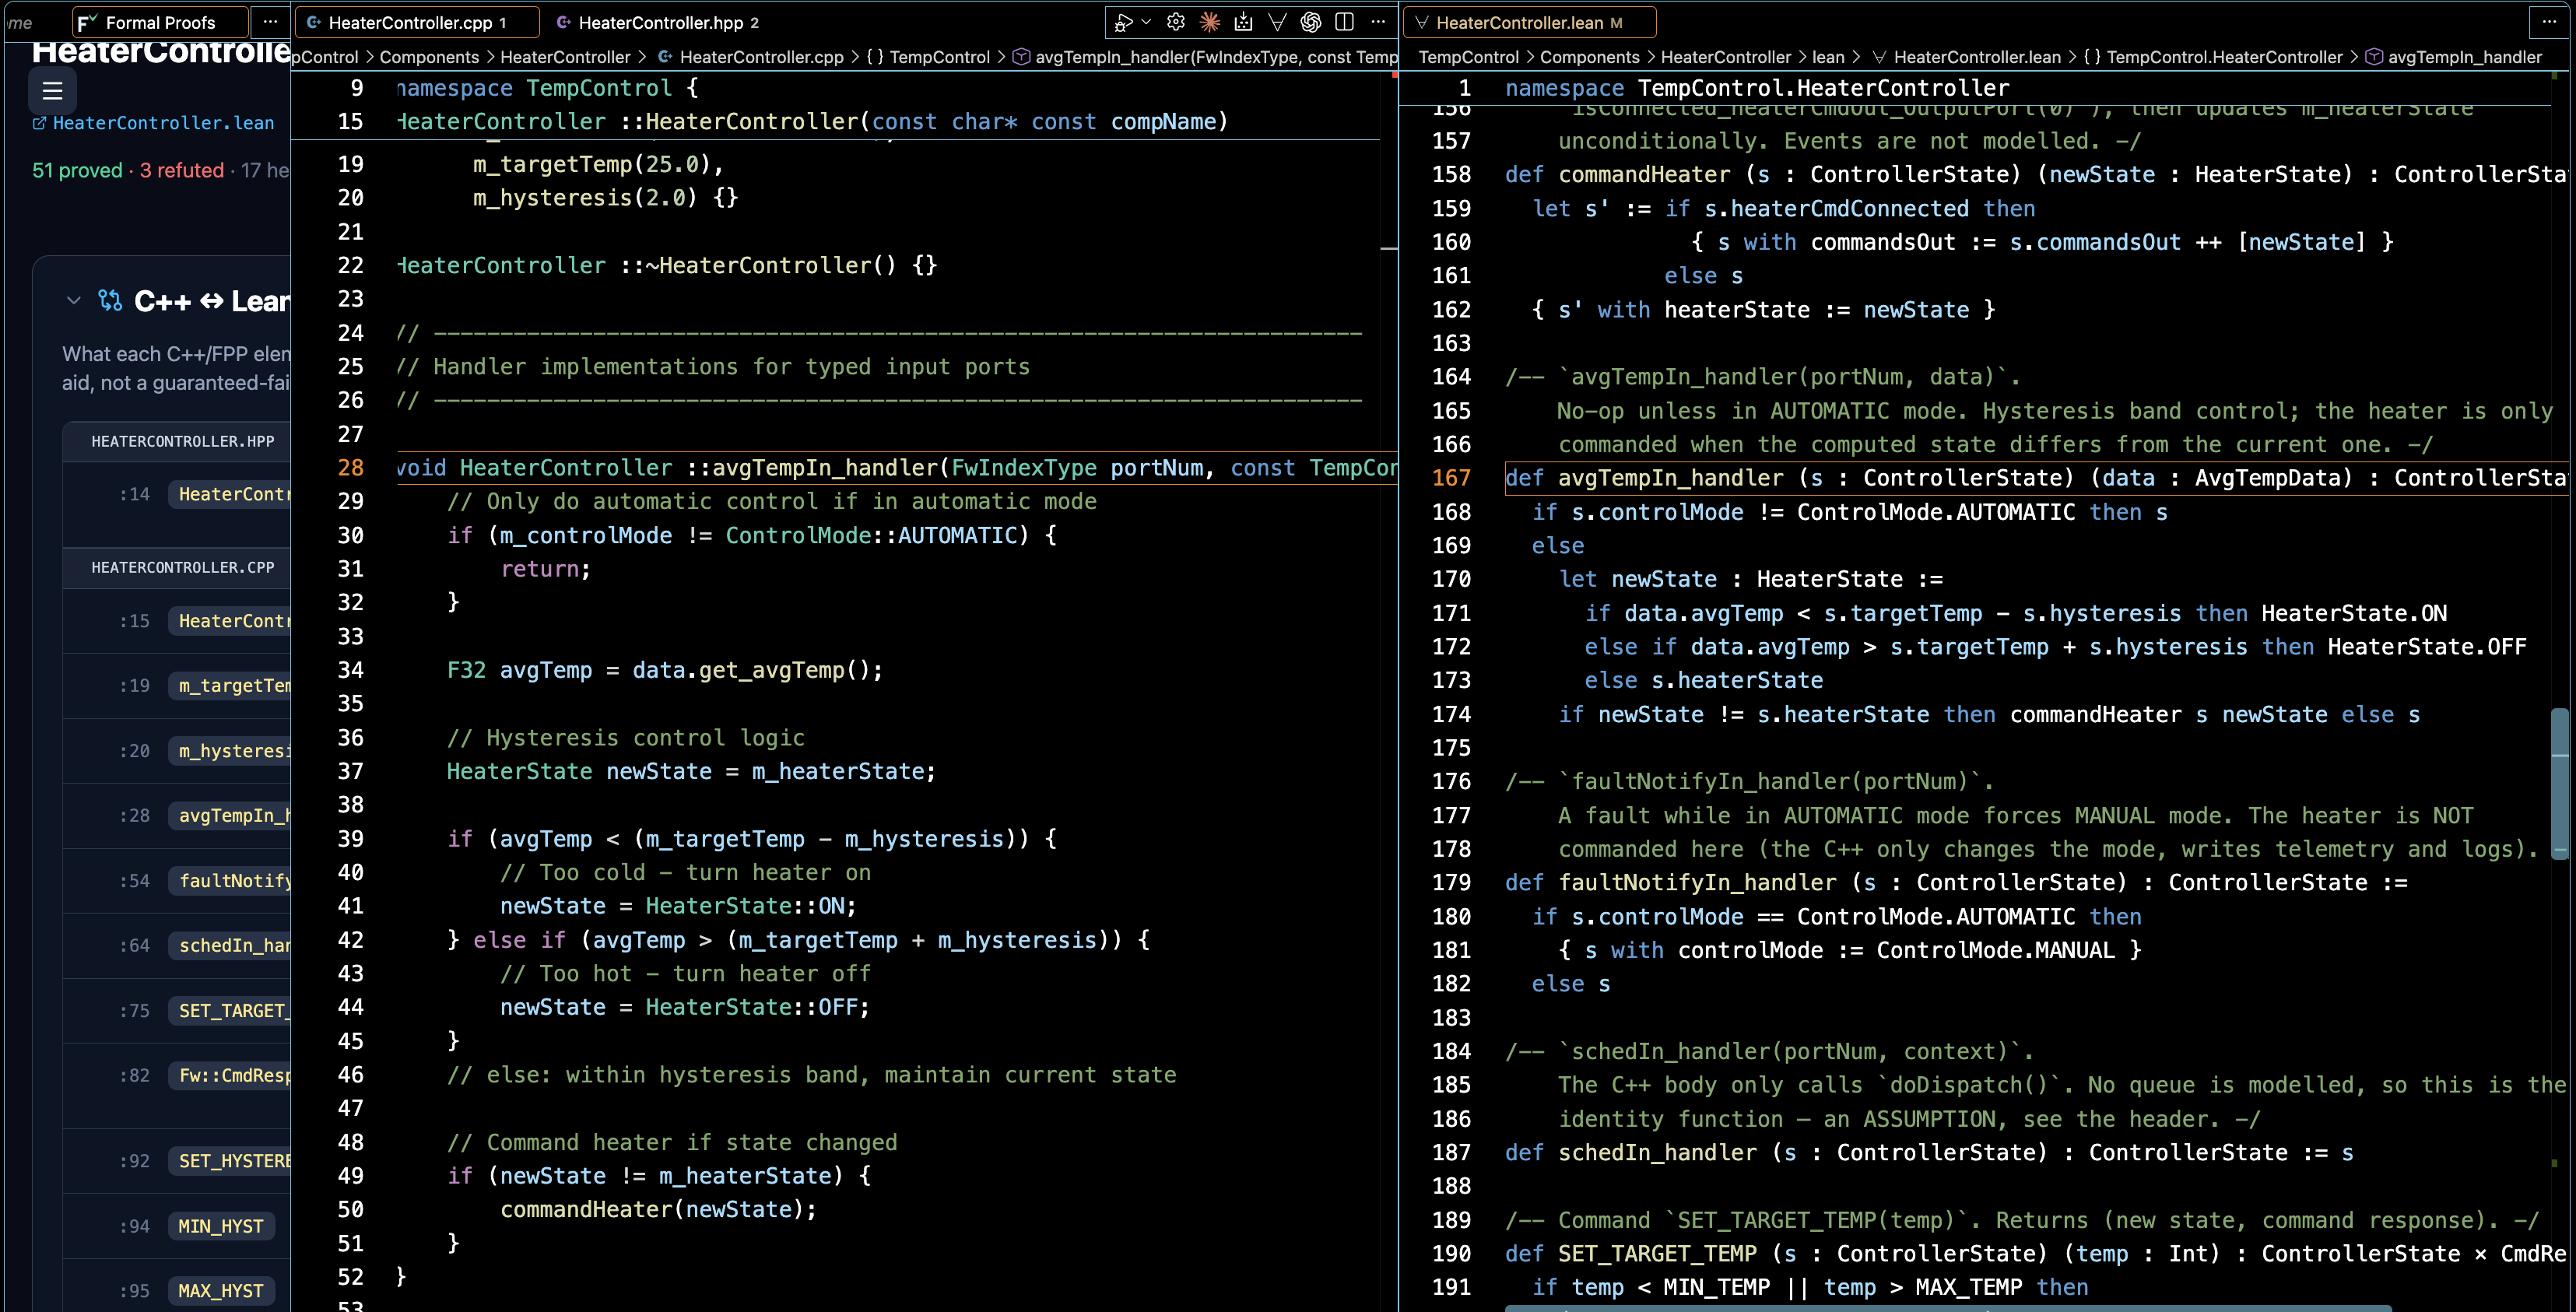
\includegraphics[width=\textwidth,height=0.74\textheight,keepaspectratio]{figures/9-handler.png}\par}

\vspace{0.1cm}
{\scriptsize {\tt avgTempIn\_handler} in C++ and in \lean{}: the model tracks the code line for line.}

\end{frame}

%----------------------------------------
\begin{frame}
  \frametitle{Properties, grouped by C++ entry point} \small

\vspace{-0.15cm}
{\centering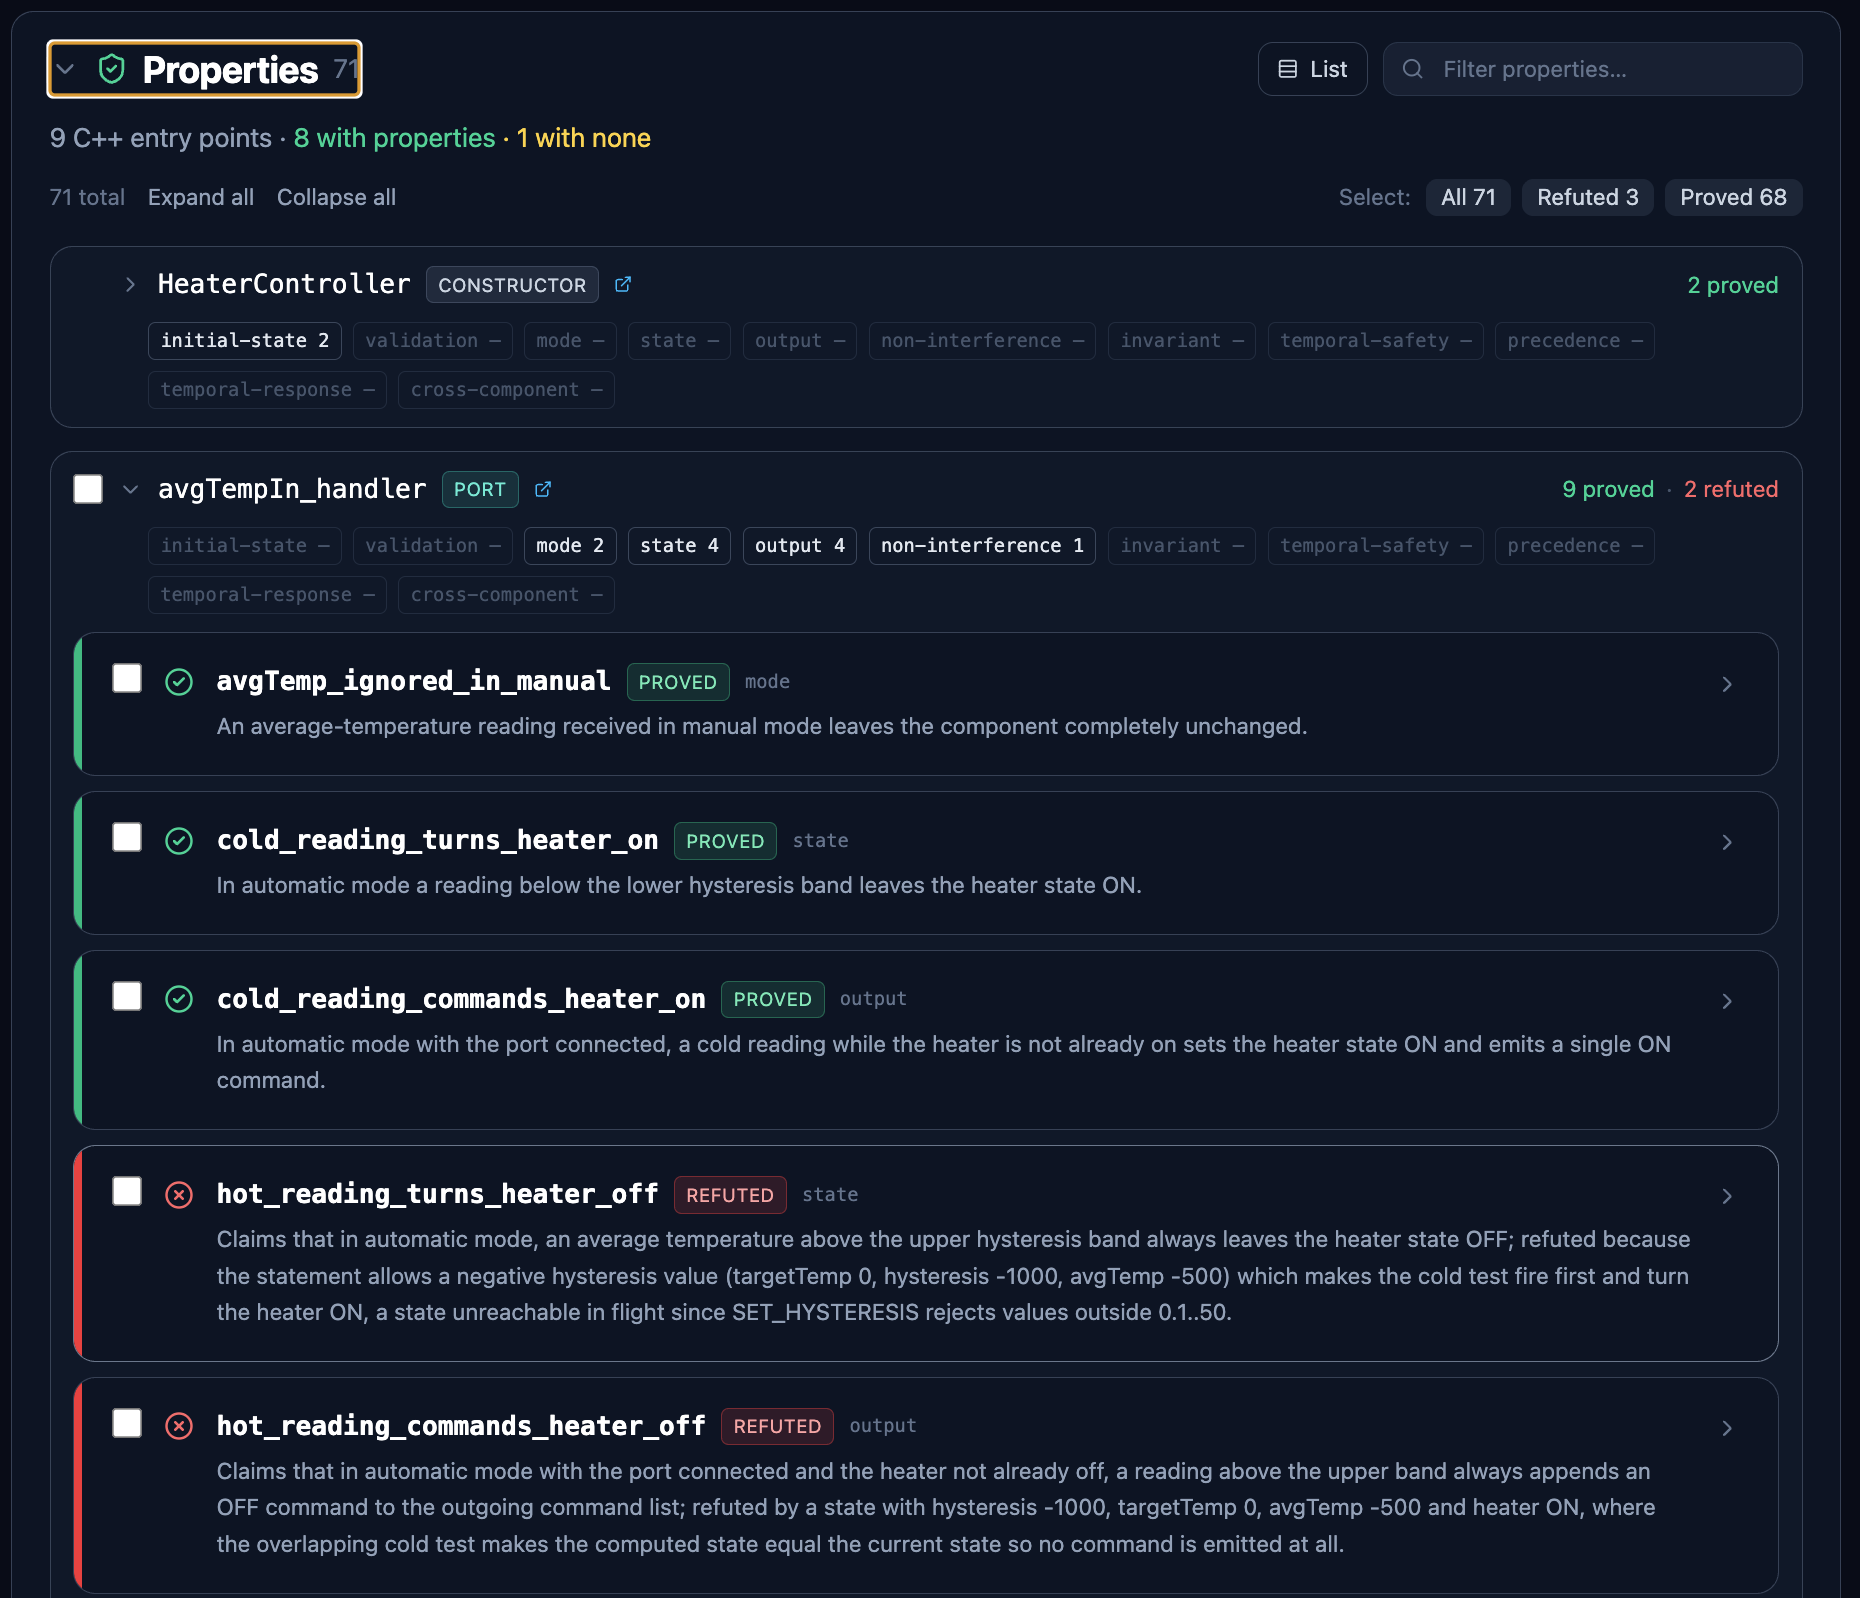
\includegraphics[width=\textwidth,height=0.74\textheight,keepaspectratio]{figures/10-properties.png}\par}

\vspace{0.1cm}
{\scriptsize Each with its English, its kind and its status. Two of these are refuted.}

\end{frame}

%----------------------------------------
\begin{frame}
  \frametitle{A refuted property, expanded} \small

\vspace{-0.15cm}
{\centering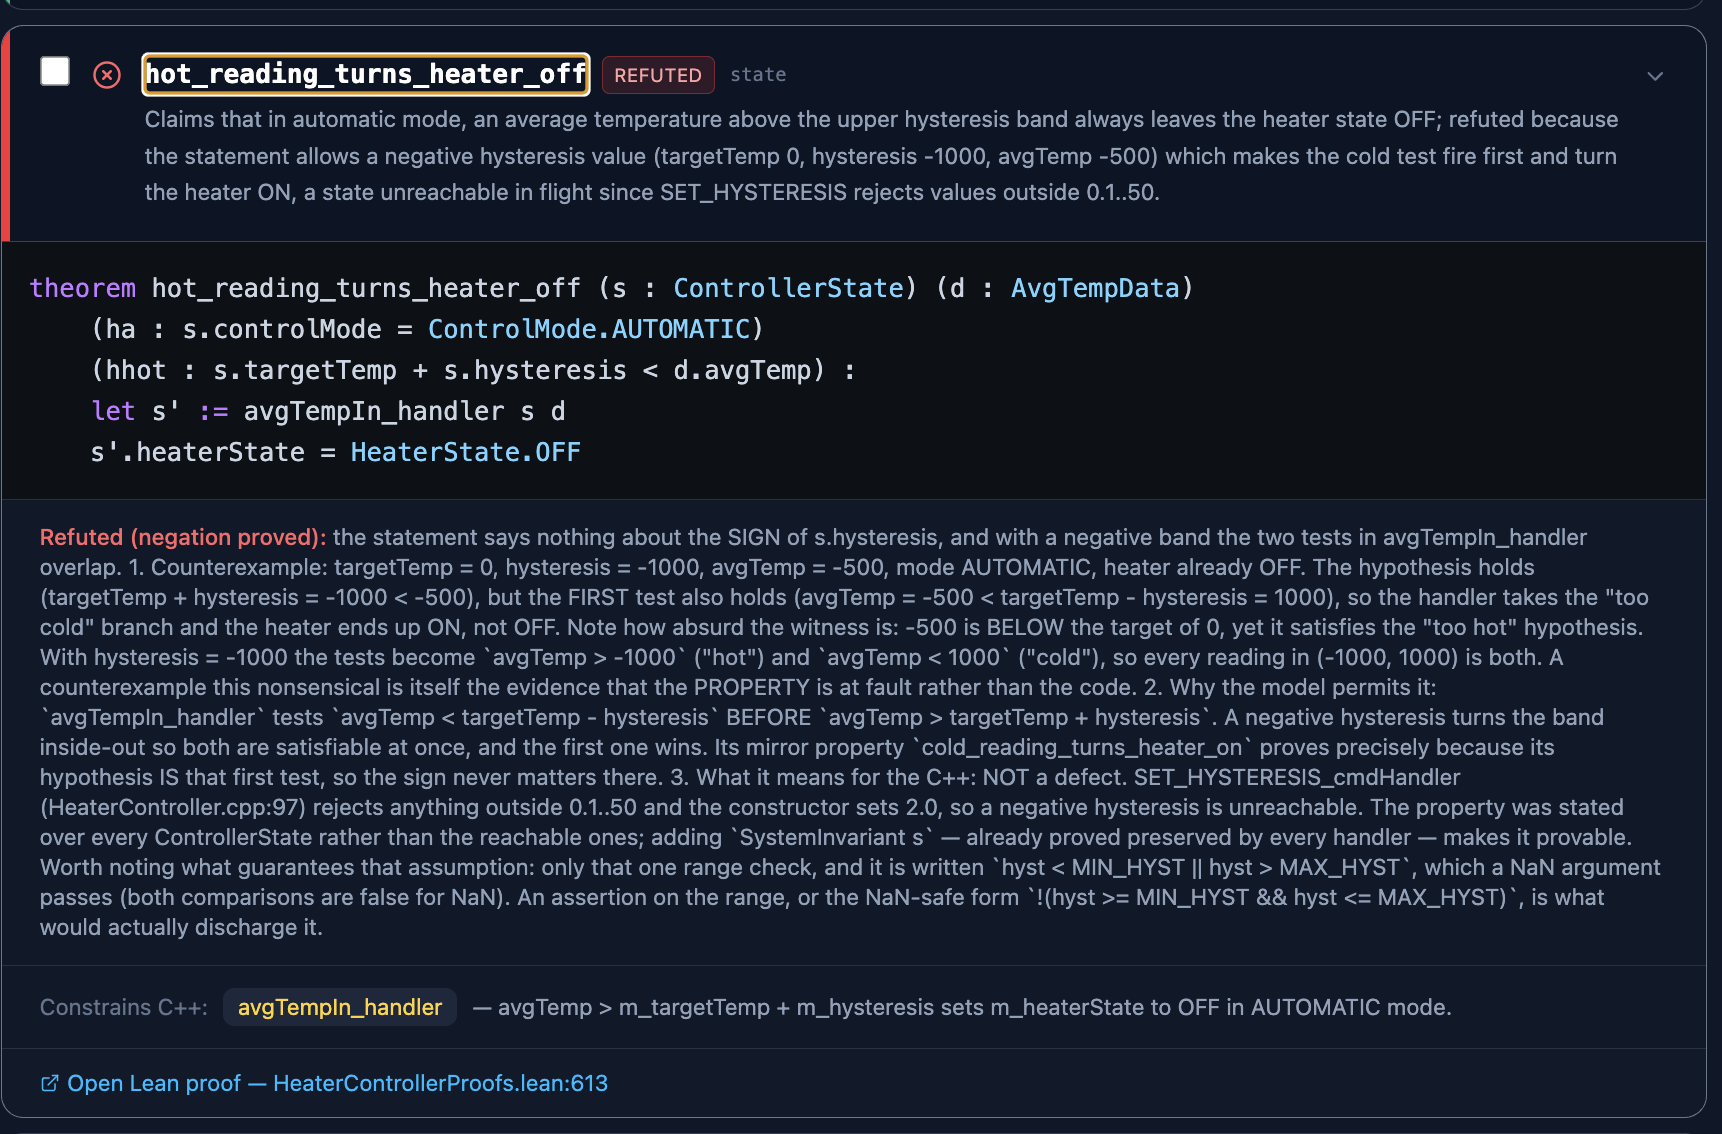
\includegraphics[width=\textwidth,height=0.73\textheight,keepaspectratio]{figures/11-lean-heater-off.png}\par}

\vspace{0.1cm}
{\scriptsize The statement, the counterexample, why the model allows it, and what it means
for the C++.}

\end{frame}
